\documentclass[a4paper,11pt,UTF8]{article}
\usepackage{ctex}
\usepackage{amsmath,amsthm,amssymb,amsfonts}
\usepackage{amsmath}
\usepackage[a4paper]{geometry}
\usepackage{graphicx}
\usepackage{microtype}
\usepackage{siunitx}
\usepackage{booktabs}
\usepackage[colorlinks=false, pdfborder={0 0 0}]{hyperref}
\usepackage{cleveref}
\usepackage{esint} 
\usepackage{graphicx}
\usepackage{ragged2e}
\usepackage{pifont}
\usepackage{extarrows}
\usepackage{mathptmx}
\usepackage{float}
\usepackage{caption}
\usepackage{subfigure}
\captionsetup[figure]{name={图}}
%opening
\title{数字电子技术作业(三)}
\author{谢悦晋 \quad U202210333}
\date{Oct 23rd, 2023 }
\begin{document}
\maketitle
\textbf{4.4.9} 试用74HC138和必要的与非门,设计一个乘法器电路,实现两位二进制数相乘,并输出结果。

\textbf{4.4.12} 图题 4.4.12 所示为 8×8 个 LED 阵列显示示意图。3 线-8 线译码器控制逐行扫描, 从上到下每次显示一行。存储阵列共有8×8 个存储单元,每个单元存放 1位显示的数据,需要显示的点存 1,否则存 0。地址线 $W_2W_1W_0$ 从 000 到 111 变化时,每次将一组 8 个数据送到输出端,控制发光二极管,需要发光的二极管接 1,否则接 0。如要显示的字形如图题 4.4.12(b)所示, 试写出存储器存放的数据。若人的视觉暂留时间为 0.05 s,在满足 LED 阵列图像稳定不闪烁的情况下,试计算地址变换的最低频率。
\begin{figure}[H]
	\centering
	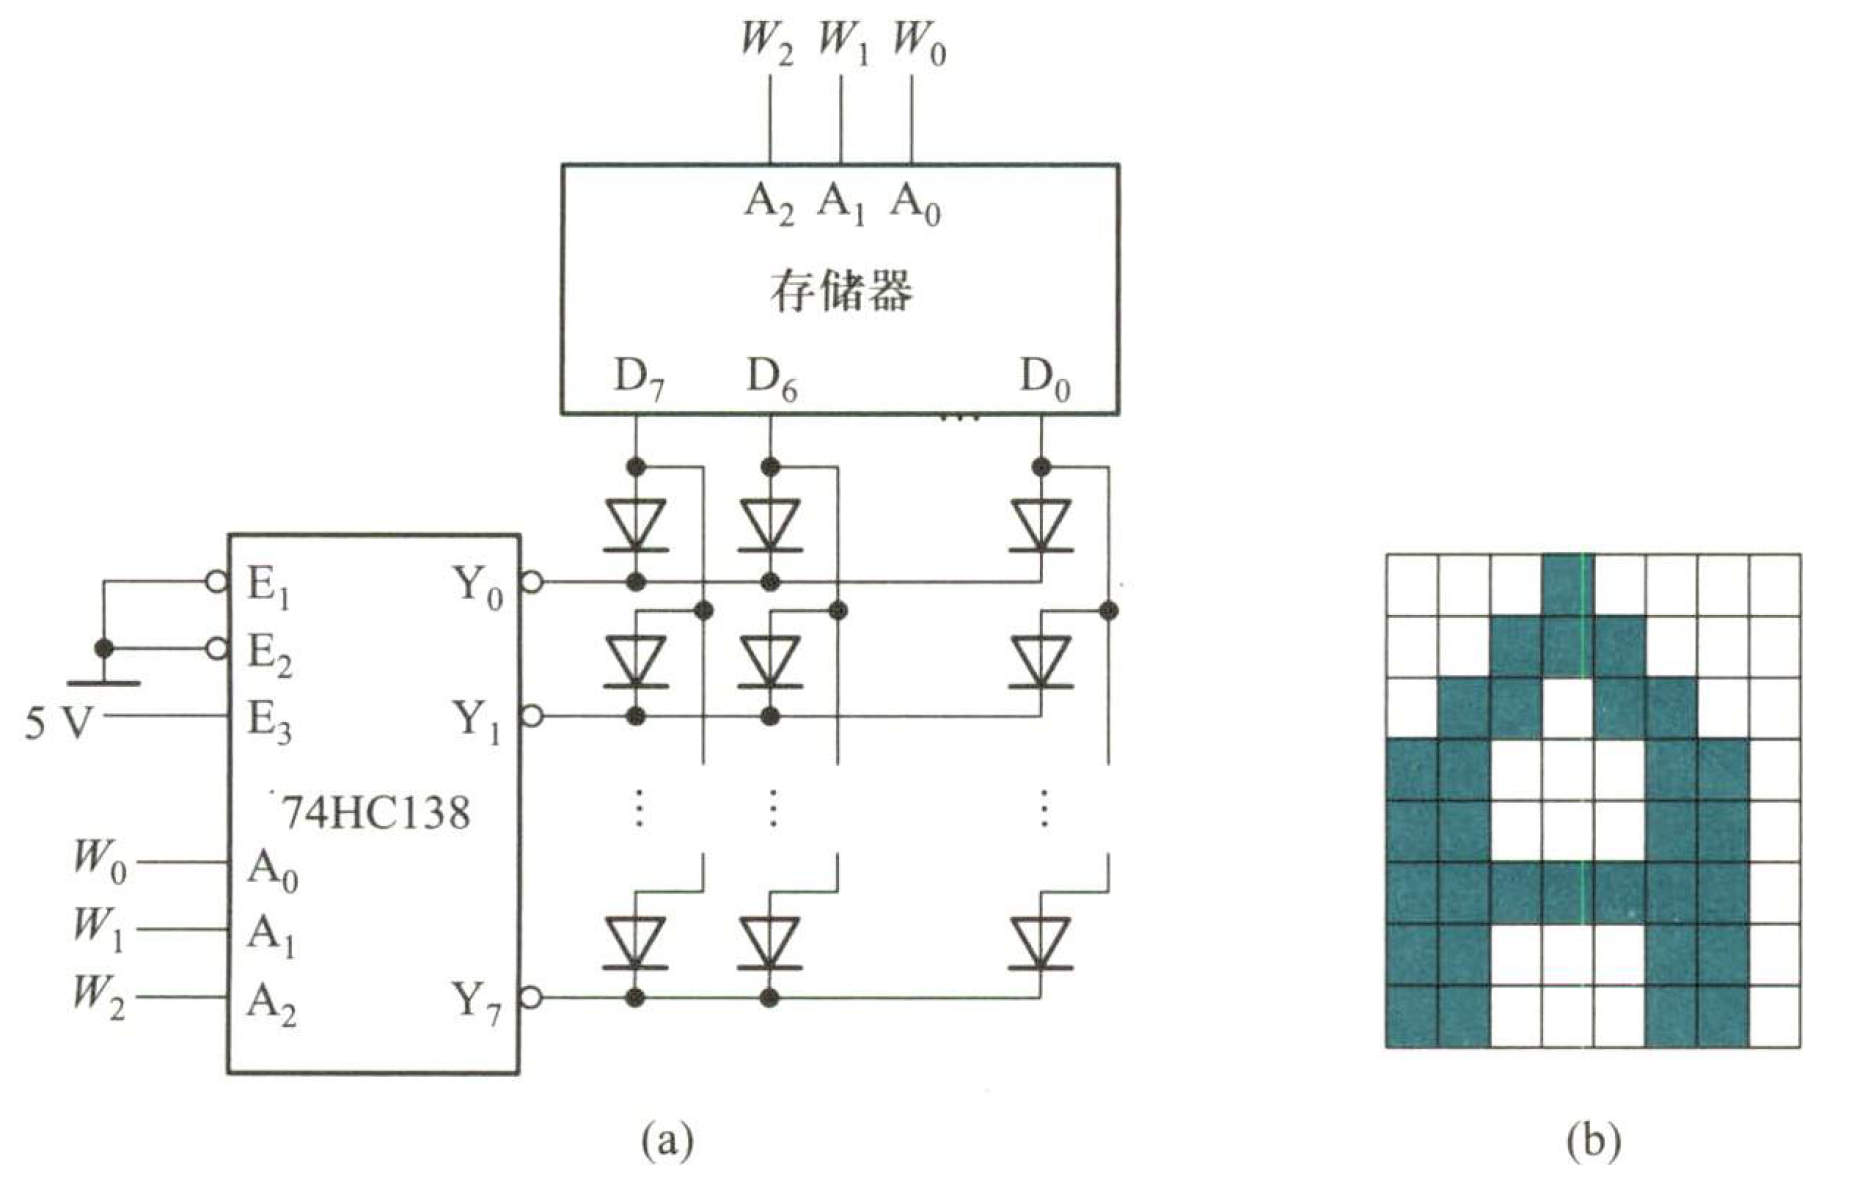
\includegraphics[width=1\textwidth]{4.4.12}
\end{figure}
\textbf{4.4.20} 试用4选1数据选择器产生下列逻辑函数:

$(1)L(A,B)=\overline{A}\cdot\overline{B}+AB$

$(2)L(A,B,C)=\sum m(1,2,6,7)$

\textbf{4.4.23}具有低使能控制的8选1数据选择器(74HC151,$\overline{E}={1}$ 时,$Y={0}$)构成的电路和各输入端的输入波形如图题 4.4.23 所示,画出输出端 $Y$ 的波形。
\begin{figure}[H]
	\centering
	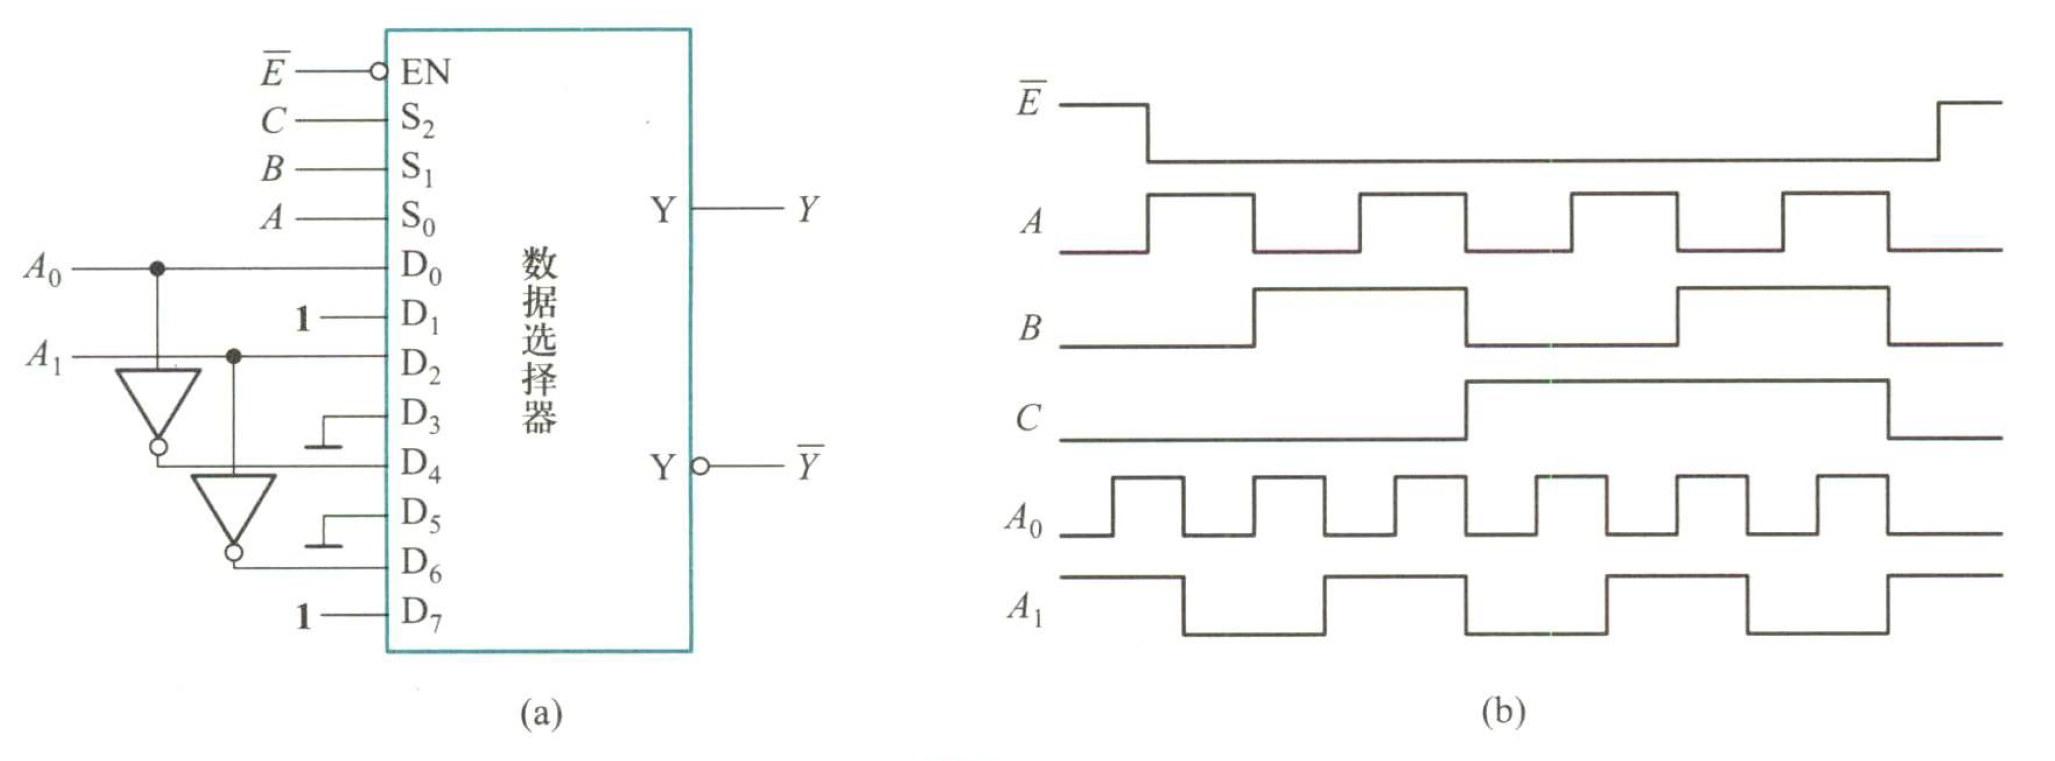
\includegraphics[width=1\textwidth]{4.4.23}
\end{figure}
\textbf{4.4.35} 仿照半加器和全加器的设计方法,试设计一半减器和一全减器,所用的门电路由自己选定。

\textbf{4.4.37} 逻辑电路如图题 4.4.37 所示,试分析该电路的功能
\begin{figure}[H]
	\centering
	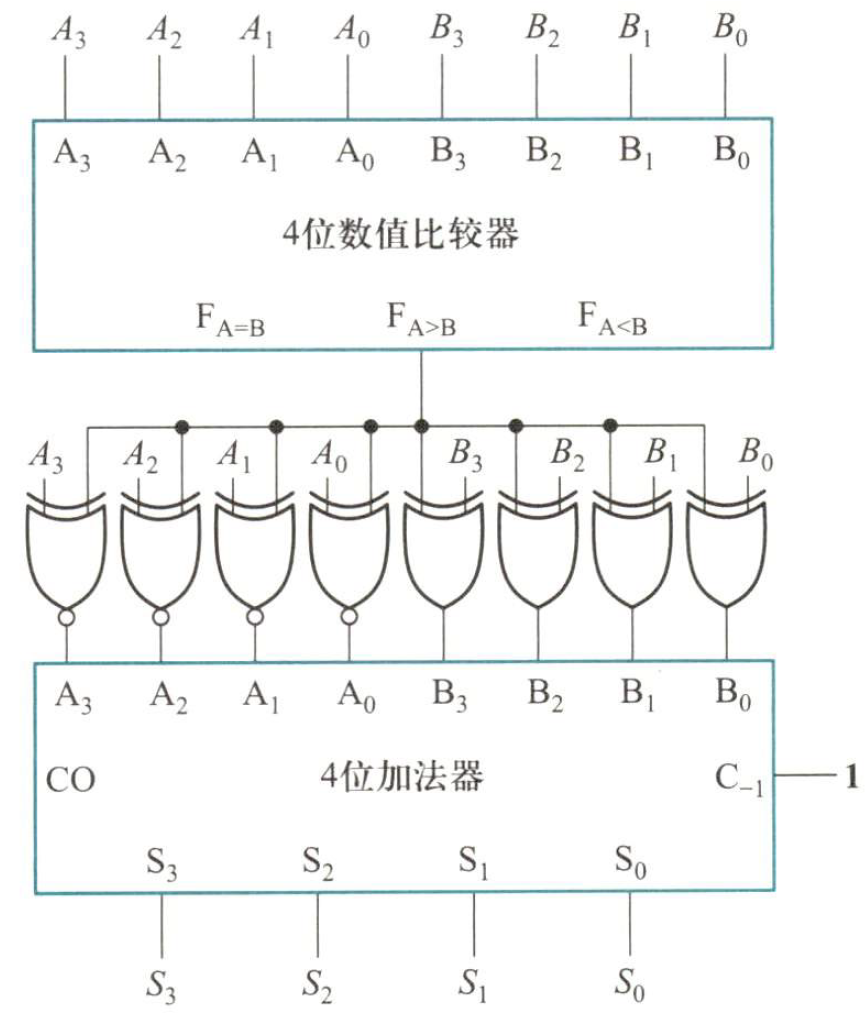
\includegraphics[width=0.5\textwidth]{4.4.37}
	\caption{}
\end{figure}
\end{document}